
\chapter{Introduction}
\label{chapter:introduction}

At the end of Dennard scaling, it may be tempting to think that VLSI and digital design are becoming less-important engineering fields.
However, the United States government wouldn't agree, considering they are investing \$280 billion over the next ten years into the CHIPS Act \cite{mckinsey}.
Similarly, TSMC, the world's leading semiconductor manufacturer, is expecting to open three new advanced-node fabs in 2024 \cite{taipeitimes}.
In addition, in 2020, Google started a partnership with GlobalFoundries, SkyWater Technology, and Efabless to provide fully open-source Process Design Kits (PDKs) and tool-chains to lower the barrier of entry for new Silicon engineers \cite{GooglePartnersWithSkyWater, googleSilicon}.
Investments like these have created a never-ending demand for chip developers, and Universities should be working to meet this demand.


\begin{figure}[t]
    \centering
    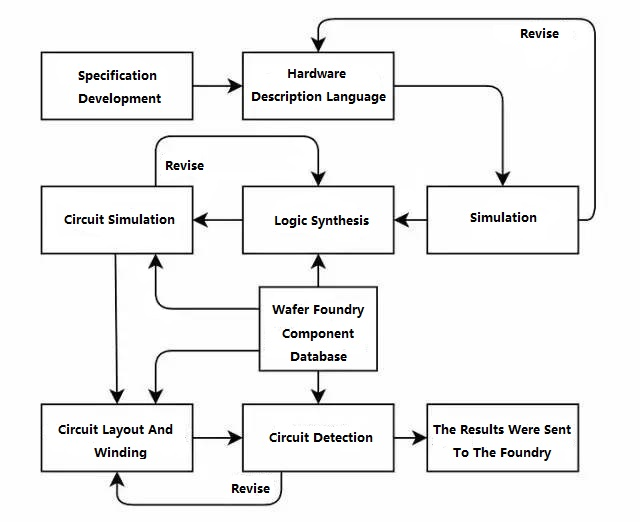
\includegraphics[width=90mm]{media/asic_flow.jpg}
    \caption{Abbreviated diagram of ASIC design flow published by Kynix \cite{kynixDesignFlow}}
    \label{fig:asic_flow}
\end{figure}


In the semiconductor industry, the process of designing an application-specific integrated circuit (ASIC) follows a well-defined sequence, where each step requires extensive training and practice \cite{intelDesignFlow, anysiliconDesignFlow, kynixDesignFlow}.
The following presents an abbreviated flow tailored for students and open-source tool usage, as illustrated in \autoref{fig:asic_flow}.
This process begins with the design phase, where engineers specify the functionality and requirements of the finished integrated circuit (IC).
Then, they use hardware description languages (HDLs) like SystemVerilog to detail the circuit's operations and verify its correctness through simulation.
After the HDL implementation passes a series of behavioral simulations, it is synthesized for the target's standard cell library and paired with additional digital and mixed-signal IP blocks.
Further testing can include running logical equivalence checks (LECs) to ensure the synthesized netlist is correct, rerunning the behavioral simulations on the synthesized netlist to check for reset behavior, or by running intensive simulations on a Field Programmable Gate Array (FPGA).
Once these circuit-level tests pass, layout is completed according to timing constraints and design rule checks (DRC).
If timing cannot be met, the layout or HDL implementation may need to be adjusted.
Finally, after the layout and simulations checks pass, the design is converted into a Graphic Data Stream (GDS) file which is sent to a semiconductor foundry for mass-production.

Because of the multitude of skills are required to create an ASIC design, it is crucial for Universities to offer a strong foundation in writing and working with HDLs to design hardware.
Nevertheless, HDLs come with a formidable learning curve, partly due to the difficulties of distinguishing between what code is synthesizable (able to be converted into hardware) and what should be used solely for verification purposes.
Additionally, the prevalence of bugs in common HDL tools, the extraordinary inaccessibility of proprietary tools, and the lack of reliable online educational resources can be a major deterrent for students and hobbyists who wish to experiment with digital design on their own.
Another factor contributing to the complexity is the interdisciplinary nature of ASIC design.
For many students, especially those with a software background, this may be their first experience with hardware design, while hardware students may also be transitioning into a more software-centric environment.
Bridging the gap between hardware and software is vital in today's world due to the prevalence of computer-aided design (CAD) software.
Universities must recognize the formidable learning curve associated with HDLs and provide comprehensive educational resources, practical hands-on experiences, and interdisciplinary exposure to prepare students for the intricate realm of ASIC design.

To aid educators in combating the intrinsic difficulty in teaching digital design, this thesis presents a collection of methods and resources for Verilog education that will adequately prepare students for writing synthesizable Verilog in industry.

\begin{itemize}

    \item \autoref{chapter:open_source_tools} delves into the accessibility of open-source tools, highlighting how they provide a cost-effective alternative for students, unlike proprietary tools burdened with high licensing fees.
    It also discusses the ease of installation and the unique features offered by open-source tools, emphasizing their ability to foster a more exciting and accessible learning environment.

    \item \autoref{chapter:digital_design} shifts the focus to teaching SystemVerilog from a synthesis perspective, and how SystemVerilog can be effectively used for digital design education.
    It argues that a synthesis-oriented approach to teaching SystemVerilog can bridge the gap between abstract syntax and tangible hardware implementations, providing students with a deeper understanding of digital circuits.

    \item \autoref{chapter:resources} explores the best resources for learning synthesizable SystemVerilog.
    It argues the significance of SystemVerilog style guides in ensuring code quality and adherence to industry standards while warning against relying solely on popular yet misleading Verilog tutorial websites.

    \item \autoref{chapter:scalability} emphasizes the importance of teaching students how to efficiently work on large-scale Verilog projects, discussing features in SystemVerilog that aid in code organization, and the significance of version control and in-module verification.

    \item \autoref{chapter:autograders} argues for the incorporation of autograders in Verilog/SystemVerilog education, demonstrating their value in providing instant, high-quality feedback to students.
    It also discusses how autograders can facilitate remote testing of Verilog designs and foster a sense of community and collaboration among students.

    \item \autoref{chapter:labs_with_cva6} culminates the thesis by showcasing a series of assignments I created that provide hands-on experience with advanced computer architecture concepts using the open-source CVA6 RISC-V core.

    \item Finally, \autoref{chapter:other_classes} explores how ideas presented in this thesis could enhance additional advanced Verilog courses such as verification with Universal Verification Methodology (UVM) and SystemVerilog Assertions (SVA) for verification, embedded system and System-on-Chip (SoC) design, and ASIC and VLSI projects.

\end{itemize}
